

\noindent
Zur Überprüfung der in Abschnitt~3.2 durchgeführten Zerlegung werden die ursprüng-
liche Funktion $f(x)$ sowie deren gerader und ungerader Anteil grafisch dargestellt.
Ziel ist es, die mathematische Zerlegung anhand der Graphen zu verifizieren.
\begin{figure}[H]
    \centering
    
\includegraphics[width=1\textwidth]{3_3_g_h_sum.png}
    \caption{Alle Funktionen einzeln geplotet}
    \label{fig:Alle Funktionen einzeln geplotet}
\end{figure}

\noindent
Zunächst werden die Funktionen $g(x)$ und $h(x)$ getrennt geplottet. Dabei zeigt
sich, dass der Graph des geraden Anteils $g(x)$ achsensymmetrisch zur y-Achse
verläuft, während der ungerade Anteil $h(x)$ punktsymmetrisch zum Ursprung ist.
Dies entspricht exakt den theoretischen Eigenschaften gerader und ungerader
Funktionen.
\begin{figure}[H]
    \centering
    \begin{subfigure}{0.48\textwidth}
        \centering
        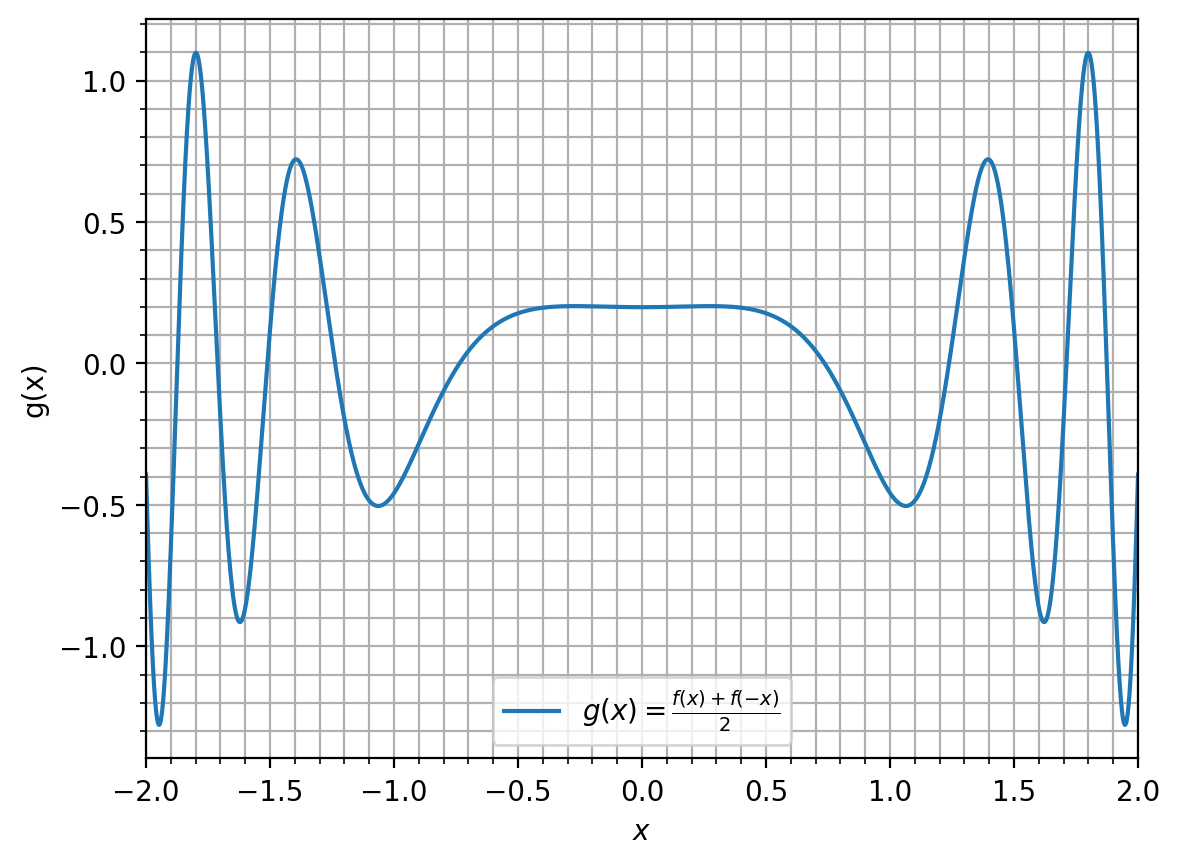
\includegraphics[width=\linewidth]{pictures/3_3_g_only.png}
        \caption{Funktion $g(x)$}
        \label{fig:g}
    \end{subfigure}
    \hfill
    \begin{subfigure}{0.48\textwidth}
        \centering
        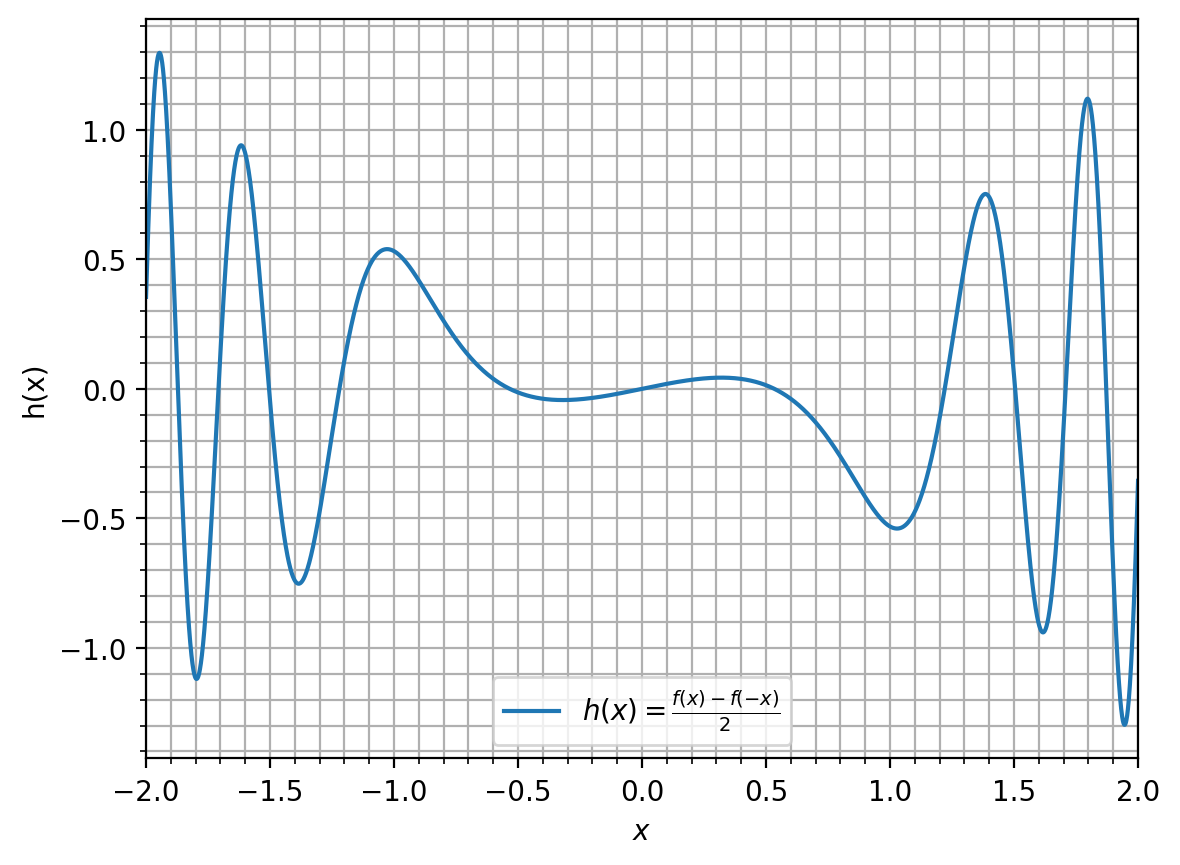
\includegraphics[width=\linewidth]{pictures/3_3_h_only.png}
        \caption{Funktion $h(x)$}
        \label{fig:h}
    \end{subfigure}
    \caption{Graphen der Funktionen $g$ und $h$}
    \label{fig:g_h}
\end{figure}



\noindent
Anschließend wird die Summe der beiden Teilfunktionen $g(x) + h(x)$ grafisch
dargestellt und mit der ursprünglichen Funktion $f(x)$ verglichen. Dabei ist
festzustellen, dass beide Graphen deckungsgleich sind.
\begin{figure}[H]
    \centering
    
\includegraphics[width=1\textwidth]{3_3_f_vs_g_plus_h.png}
    \caption{Plot zum Vergleichen der Funktionen}
    \label{fig:Plot zum Vergleichen der Funktionen}
\end{figure}

\noindent
Damit wird bestätigt, dass die in Abschnitt~3.2 durchgeführte Zerlegung korrekt ist
und die ursprüngliche Funktion vollständig durch die Summe ihres geraden und
ungeraden Anteils beschrieben wird.
